\documentclass{article}

\usepackage[utf8]{inputenc}  %Kodna stran za Windows okolje, za linux je kodna stran latin2
\usepackage[slovene]{babel}    % pravila za slovensko deljenje besed
\usepackage{tikz}
\usetikzlibrary{tikzmark}
\usetikzlibrary{shapes,arrows,positioning,calc,babel}
\usepackage[europeanresistors]{circuitikz}
\usepackage{graphicx}
\usepackage{psfrag}
\usepackage{epstopdf}
\epstopdfsetup{update}
\usepackage[pdftex]{UNI-LJ-FE-Diploma} %Stil za diplome na Fakulteti za elektrotehniko (za pdfTeX v MkiTex)
\usepackage{MojiBloki}
%\usepackage[pctex]{UNI-LJ-FE-Diploma} %Stil za diplome na Fakulteti za elektrotehniko  (za pcTex)
\usepackage{pgfplots}
\usepackage{subfigure} 
\usepackage{verbatim}
\usepackage{transparent}
\usepackage{tikz-timing}
\usetikztiminglibrary[rising arrows]{clockarrows}
\usetikztiminglibrary{arrows}
\usetikzlibrary{calc}
\usepackage{makecell}%
\usetikzlibrary{babel}
\usepackage{setspace}
\pgfplotsset{compat=1.8}
\usetikzlibrary{intersections,backgrounds}
\usetikzlibrary{math,calc}
\tikzset{
	controller/.style = {draw, fill=blue!20, rectangle, minimum height=3.5em, minimum width=6em},
	subblock/.style= {draw, fill=blue!5, rectangle, minimum height=3.5em, minimum width=6em},
	pidblocks/.style = {draw, fill=green!5, rectangle, minimum height=3.5em, minimum width=6em, text width= 6em},
	sum/.style = {draw, circle, node distance=1cm, inner sep=0.15cm},
	input/.style = {coordinate},
	output/.style ={coordinate},
	block/.style = {draw, fill=white, rectangle, minimum height=2em, minimum width=2em},
	pinstyle/.style ={pin edge={to-,thin,black}},
	dot/.style  = {anchor=base,fill,circle,inner sep=1pt}
}
	
\tikzset{%
	saturation block/.style={%
		draw, minimum size = 0.3cm,
		path picture={
			% Get the width and height of the path picture node
			\pgfpointdiff{\pgfpointanchor{path picture bounding box}{south west}}%
			{\pgfpointanchor{path picture bounding box}{north east}}
			\pgfgetlastxy\x\y
			% Scale the x and y vectors so that the range
			% -1 to 1 is slightly shorter than the size of the node
			\tikzset{x=\x*.4, y=\y*.4}
			%
			% Draw annotation
			\draw [very thin] (-1,0) -- (1,0) (0,-1) -- (0,1); 
			\draw [very thick] (-1,-.7) -- (-.7,-.7) -- (.7,.7) -- (1,.7);
		},
		append after command={\pgfextra{\let\mainnode=\tikzlastnode}
			node[above right] at (\mainnode.north west) {#1}%
		}	
	}
}
	
\tikzset{%
	Filt block/.style = {%
		draw, minimum size = 0.8cm,
		path picture={
			% Get the width and height of the path picture node
			\pgfpointdiff{\pgfpointanchor{path picture bounding box}{south west}}%
			{\pgfpointanchor{path picture bounding box}{north east}}
			\pgfgetlastxy\x\y
			% Scale the x and y vectors so that the range
			% -1 to 1 is slightly shorter than the size of the node
			\tikzset{x=\x*.4, y=\y*.4}
			%
			% Draw annotation
			\draw [very thin] (-1,-1) -- (-1,1) (-1,-1) -- (1,-1); 
			\draw [very thick] (-0.95, -1) arc  [x radius =1.9, y radius = 1.4, start angle = 180,  end angle = 90] ;
		},
		append after command={\pgfextra{\let\mainnode=\tikzlastnode}
			node[above right] at (\mainnode.north west) {#1}%
		}
	}	
}
	
\tikzset{%
	Pctrl block/.style={%
		draw, minimum size = 0.8cm,
		path picture={
			% Get the width and height of the path picture node
			\pgfpointdiff{\pgfpointanchor{path picture bounding box}{south west}}%
			{\pgfpointanchor{path picture bounding box}{north east}}
			\pgfgetlastxy\x\y
			% Scale the x and y vectors so that the range
			% -1 to 1 is slightly shorter than the size of the node
			\tikzset{x=\x*.4, y=\y*.4}
			%
			% Draw annotation
			\draw [very thin] (-1,-1) -- (-1,1) (-1,-1) -- (1,-1); 
			\draw [very thick] (-1,.4) -- (1,.4);
		},
		append after command={\pgfextra{\let\mainnode=\tikzlastnode}
			node[above] at (\mainnode.north) {#1}%
		}	
	}
}
	
\tikzset{%
	PIctrl block/.style={%
		draw, minimum size = 0.8cm,
		path picture={
			% Get the width and height of the path picture node
			\pgfpointdiff{\pgfpointanchor{path picture bounding box}{south west}}%
			{\pgfpointanchor{path picture bounding box}{north east}}
			\pgfgetlastxy\x\y
			% Scale the x and y vectors so that the range
			% -1 to 1 is slightly shorter than the size of the node
			\tikzset{x=\x*.4, y=\y*.4}
			%
			% Draw annotation
			\draw [very thin] (-1,-1) -- (-1,1) (-1,-1) -- (1,-1); 
			\draw [very thick]   (-0.95,-1) -- (-0.95, -0.2) -- (0.9,.4);
		},
		append after command={\pgfextra{\let\mainnode=\tikzlastnode}
			node[above] at (\mainnode.north) {#1}%
		}	
	}
}
	
\tikzset{%
	Difer block/.style={%
		draw, minimum size = 0.8cm,
		path picture={
			% Get the width and height of the path picture node
			\pgfpointdiff{\pgfpointanchor{path picture bounding box}{south west}}%
			{\pgfpointanchor{path picture bounding box}{north east}}
			\pgfgetlastxy\x\y
			% Scale the x and y vectors so that the range
			% -1 to 1 is slightly shorter than the size of the node
			\tikzset{x=\x*.4, y=\y*.4}
			%
			% Draw annotation
			\draw [very thin] (-1,-1) -- (-1,1) (-1,-1) -- (1,-1); 
			\draw [very thick] (-0.97,-1) -- (-0.97, 0.6);
		},
		append after command={\pgfextra{\let\mainnode=\tikzlastnode}
			node[above right] at (\mainnode.north west) {#1}%
		}				
	}
}
	
\tikzset{%
	Integ block/.style={%
		draw, minimum size = 0.8cm,
		path picture={
			% Get the width and height of the path picture node
			\pgfpointdiff{\pgfpointanchor{path picture bounding box}{south west}}%
			{\pgfpointanchor{path picture bounding box}{north east}}
			\pgfgetlastxy\x\y
			% Scale the x and y vectors so that the range
			% -1 to 1 is slightly shorter than the size of the node
			\tikzset{x=\x*.4, y=\y*.4}
			%
			% Draw annotation
			\draw [very thin] (-1,-1) -- (-1,1) (-1,-1) -- (1,-1);  
			\draw [very thick] (-1,-1) -- (1, 1);
		},
		append after command={\pgfextra{\let\mainnode=\tikzlastnode}
			node[above] at (\mainnode.north) {#1}%
		}				
	}
}	
	
\tikzset{%
	Limit block/.style={%
		fill = none, minimum size = 0.5cm,
		path picture={
			% Get the width and height of the path picture node
			\pgfpointdiff{\pgfpointanchor{path picture bounding box}{south west}}%
			{\pgfpointanchor{path picture bounding box}{north east}}
			\pgfgetlastxy\x\y
			% Scale the x and y vectors so that the range
			% -1 to 1 is slightly shorter than the size of the node
			\tikzset{x=\x*.4, y=\y*.4}
			%
			% Draw annotation
			\draw [thick] (-1,1) -- (-0.8, 0.5) -- (0.8,0.5) -- (1,1);
			\draw [thick] (-1,-1) -- (-0.8, -0.5) -- (0.8,-0.5) -- (1,-1);
		},
		append after command={\pgfextra{\let\mainnode=\tikzlastnode}
			node[above] at (\mainnode.north) {#1}%
		}				
	}
}			

	\tikzset{%
		mul above/.style={%
			draw, minimum size = 0.3cm,
			path picture={
				% Get the width and height of the path picture node
				\pgfpointdiff{\pgfpointanchor{path picture bounding box}{south west}}%
				{\pgfpointanchor{path picture bounding box}{north east}}
				\pgfgetlastxy\x\y
				% Scale the x and y vectors so that the range
				% -1 to 1 is slightly shorter than the size of the node
			%	\tikzset{x=\x*.4, y=\y*.4}
				%
				% Draw annotation
				\draw [thick] (-1,-1) -- (1,1); 
				\draw [thick] (-1,1) -- (1,-1);
			},
			append after command={\pgfextra{\let\mainnode=\tikzlastnode}
					node[above](A1) at ([yshift=0.5cm]\mainnode.north) {#1}%
          [->] (A1) edge (\mainnode.north)			   
			},
		}
	}

		\tikzset{%
			mul below/.style={%
				draw, minimum size = 0.3cm,
				path picture={
					% Get the width and height of the path picture node
					\pgfpointdiff{\pgfpointanchor{path picture bounding box}{south west}}%
					{\pgfpointanchor{path picture bounding box}{north east}}
					\pgfgetlastxy\x\y
					% Scale the x and y vectors so that the range
					% -1 to 1 is slightly shorter than the size of the node
					%	\tikzset{x=\x*.4, y=\y*.4}
					%
					% Draw annotation
					\draw [thick] (-1,-1) -- (1,1); 
					\draw [thick] (-1,1) -- (1,-1);
				},
				append after command={\pgfextra{\let\mainnode=\tikzlastnode}
					node[below](A1) at ([yshift=-0.5cm]\mainnode.south) {#1}%
					[->] (A1) edge (\mainnode.south)			   
				},
			}
		}

\tikzset{%
	mul left/.style={%
		draw, minimum size = 0.3cm,
		path picture={
			% Get the width and height of the path picture node
			\pgfpointdiff{\pgfpointanchor{path picture bounding box}{south west}}%
			{\pgfpointanchor{path picture bounding box}{north east}}
			\pgfgetlastxy\x\y
			% Scale the x and y vectors so that the range
			% -1 to 1 is slightly shorter than the size of the node
			%	\tikzset{x=\x*.4, y=\y*.4}
			%
			% Draw annotation
			\draw [thick] (-1,-1) -- (1,1); 
			\draw [thick] (-1,1) -- (1,-1);
		},
		append after command={\pgfextra{\let\mainnode=\tikzlastnode}
			node[left](A1) at ([xshift=-0.5cm]\mainnode.west) {#1}%
			[->] (A1) edge (\mainnode.west)			   
		},
	}
}	

\tikzset{%
	mul right/.style={%
		draw, minimum size = 0.3cm,
		path picture={
			% Get the width and height of the path picture node
			\pgfpointdiff{\pgfpointanchor{path picture bounding box}{south west}}%
			{\pgfpointanchor{path picture bounding box}{north east}}
			\pgfgetlastxy\x\y
			% Scale the x and y vectors so that the range
			% -1 to 1 is slightly shorter than the size of the node
			%	\tikzset{x=\x*.4, y=\y*.4}
			%
			% Draw annotation
			\draw [thick] (-1,-1) -- (1,1); 
			\draw [thick] (-1,1) -- (1,-1);
		},
		append after command={\pgfextra{\let\mainnode=\tikzlastnode}
			node[right](A1) at ([xshift=0.5cm]\mainnode.east) {#1}%
			[->] (A1) edge (\mainnode.east)			   
		},
	}
}

\tikzset{%
	notch block/.style={%
		draw, minimum size = 0.8cm,
		path picture={
			% Get the width and height of the path picture node
			\pgfpointdiff{\pgfpointanchor{path picture bounding box}{south west}}%
			{\pgfpointanchor{path picture bounding box}{north east}}
			\pgfgetlastxy\x\y
			% Scale the x and y vectors so that the range
			% -1 to 1 is slightly shorter than the size of the node
			\tikzset{x=\x*.4, y=\y*.4}
			%
			% Draw annotation  
			\draw [very thin] (-1,-1) -- (1,-1);  
			\draw [thick] (-0.5, 0.8) arc  [x radius =0.4, y radius = 2.4, start angle = 90,  end angle =15] (-1, 0.8) -- (-0.5, 0.8)  ;
			\draw [thick] (0.5, 0.8) arc  [x radius =0.4, y radius = 2.4, start angle = 90,  end angle = 165] (1, 0.8) -- (0.5, 0.8) ;
		},
		append after command={\pgfextra{\let\mainnode=\tikzlastnode}
			node[above right] at (\mainnode.north west) {#1}%
		}				
	}
}	
\tikzset{%
	bandstop block/.style={%
		draw, minimum size = 0.8cm,
		path picture={
			% Get the width and height of the path picture node
			\pgfpointdiff{\pgfpointanchor{path picture bounding box}{south west}}%
			{\pgfpointanchor{path picture bounding box}{north east}}
			\pgfgetlastxy\x\y
			% Scale the x and y vectors so that the range
			% -1 to 1 is slightly shorter than the size of the node
			\tikzset{x=\x*.4, y=\y*.4}
			%
			% Draw annotation  
			\draw [very thin] (-1,-1) -- (1,-1);  
			\draw [thick] (-0.5, 0.8) arc  [x radius =0.8, y radius = 1.8, start angle = 90,  end angle =0] (-1, 0.8) -- (-0.5, 0.8)  ;
		},
		append after command={\pgfextra{\let\mainnode=\tikzlastnode}
			node[above right] at (\mainnode.north west) {#1}%
		}				
	}
}

\tikzset{
	old inner xsep/.estore in=\oldinnerxsep,
	old inner ysep/.estore in=\oldinnerysep,
	double circle/.style 2 args={fill=black, even odd rule,
		circle,
		old inner xsep=\pgfkeysvalueof{/pgf/inner xsep},
		old inner ysep=\pgfkeysvalueof{/pgf/inner ysep},
		/pgf/inner xsep=\oldinnerxsep+#1,
		/pgf/inner ysep=\oldinnerysep+#1,
		alias=sourcenode,
		append after command={
			let     \p1 = (sourcenode.center),
			\p2 = (sourcenode.east),
			\n1 = {\x2-\x1-#1-0.5*\pgflinewidth}
			in
			node [inner sep=0pt, draw, circle, minimum width=2*\n1,at=(\p1),#2] {}
		}
	},
	double circle/.default={2pt}{blue}
}

\tikzset{%
	traj block/.style={%
		draw, minimum size = 3cm,
		path picture={
			% Get the width and height of the path picture node
			\pgfpointdiff{\pgfpointanchor{path picture bounding box}{south west}}%
			{\pgfpointanchor{path picture bounding box}{north east}}
			\pgfgetlastxy\x\y
			% Scale the x and y vectors so that the range
			% -1 to 1 is slightly shorter than the size of the node
			\tikzset{x=\x*.4, y=\y*.4}
			%
			% Draw annotation  
			\draw [ultra thick] (-1,-0.7) -- (-0.5,0.7) -- (0.5,0.7) -- (1,-0.7);  
		},
		append after command={\pgfextra{\let\mainnode=\tikzlastnode}
			node[above right] at (\mainnode.north west) {#1}%
		}				
	}
}

\tikzset {
	convert/.style 2 args={
		minimum size=1cm,
		rounded corners=5pt,
		append after command={
			\pgfextra{
				\pgfinterruptpath
				\path (\tikzlastnode.north west)
				node[inner sep=2pt,anchor=north west]{#1};
				\path (\tikzlastnode.south east)
				node[inner sep=2pt,anchor=south east]{#2};
				\draw ([shift={(1mm, 1mm)}]\tikzlastnode.south west)
				-- ([shift={(-1mm, -1mm)}]\tikzlastnode.north east);
				\endpgfinterruptpath
			}
		},
	}
}

\tikzset{%
	set gear dots/.style={
		gear dots/.style={dash pattern=on 4pt off 4pt, dash phase=#1}},
	set gear dots=0pt,
	pics/gears/.style args={size #1 at (#2,#3) and size #4 at (#5,#6)}{code={
			\tikzmath{%
				\r1 = #1/2; \r2 = #4/2;
				\gm = atan2(#3-#6, #2-#5);
				\th = acos((\r1 == \r2) ? 0 : (\r2-\r1) / veclen(#5-#2, #6-#3));
				coordinate \c, \t;
				\c1 = (#2, #3); \t1 = (\c1) + (360-\th+\gm:\r1);
				\c2 = (#5, #6); \t2 = (\c2) + (\th+\gm:\r2);
			}
			\draw [black!80, thick, fill=gray!25] (\c1) circle [radius=\r1];
			\draw [black!80, thick, fill=gray!25] (\c2) circle [radius=\r2];
			\draw [gray, ultra thick, postaction={draw=gray!50, gear dots, ultra thick}] 
			(\t2) arc (\th+\gm:360-\th+\gm:\r2) -- 
			(\t1) arc (360-\th+\gm:360+\th+\gm:\r1) -- cycle;
		}}}




\begin{document}
	
	\begin{figure}[h]
		\centering
		\resizebox{\textwidth}{!}{%
			
			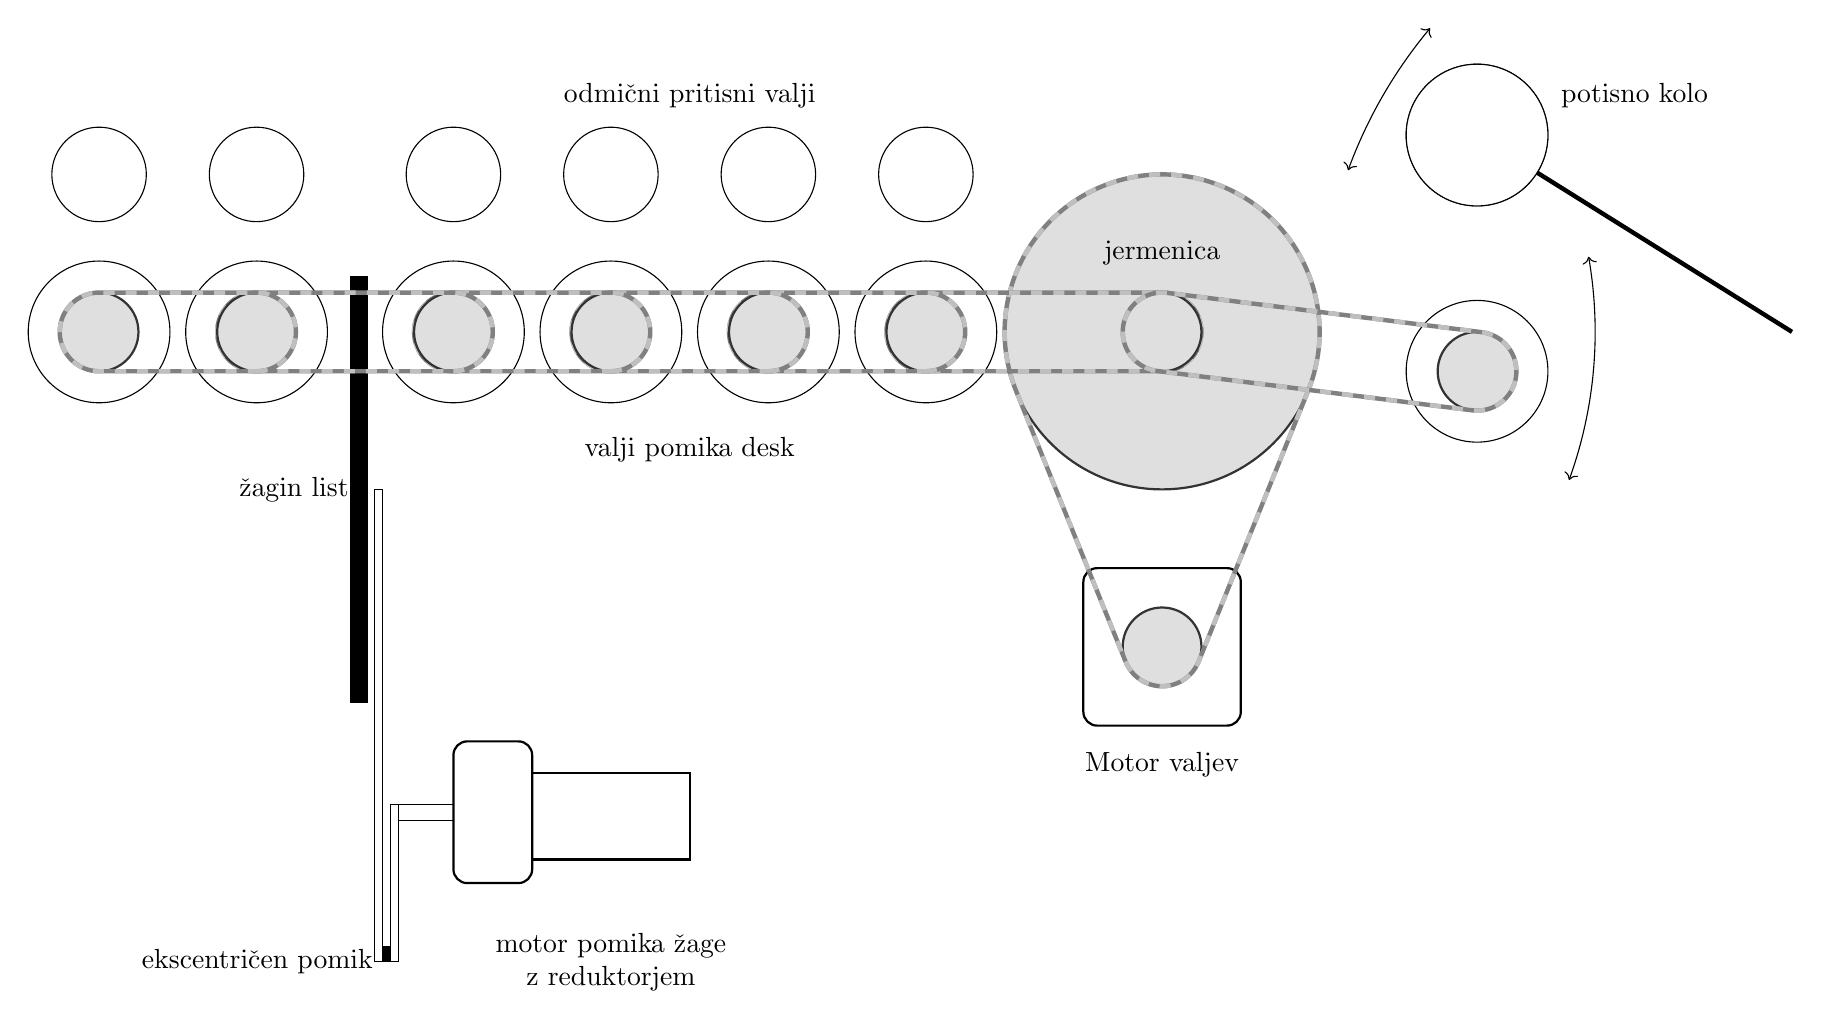
\begin{tikzpicture}
			\draw [ thick, rounded corners=5pt]  (5,-1) rectangle (7,-3);
			\draw[black,radius=0.9](3,2) circle; 
			\draw[black,radius=0.9](1,2) circle; 
			\draw[black,radius=0.9](-1,2) circle; 
			\draw[black,radius=0.9](-3,2) circle;
			\draw[black,radius=0.9](-5.5,2) circle;
			\draw[black,radius=0.9](-7.5,2) circle;   
			\draw[black,radius=0.9](10,1.5) circle;   
			\draw[black,radius=0.9](10,4.5) circle;   
			
			\draw[black,radius=0.6](3,4) circle; 
			\draw[black,radius=0.6](1,4) circle; 
			\draw[black,radius=0.6](-1,4) circle; 
			\draw[black,radius=0.6](-3,4) circle;
			\draw[black,radius=0.6](-5.5,4) circle;
			\draw[black,radius=0.6](-7.5,4) circle;   
			
			\draw [ thick, fill=black]  (-4.1,-2.7) rectangle (-4.3,2.7) node[midway, left]{žagin list};
			\draw []  (-4,0) rectangle (-3.9,-6) node[ left]{ekscentričen pomik};
			\draw []   (-3.8,-6) rectangle (-3.7,-4);
			\draw [fill=black]   (-3.9,-6) rectangle (-3.8,-5.8);
			\draw []  (-3.7,-4) rectangle (-3,-4.2);
			\draw [ thick, rounded corners=5pt]  (-3,-5) rectangle (-2,-3.2);
			\draw [ thick]  (-2,-4.7) rectangle (0,-3.6);
			\draw[-,black, ultra thick](10,4.5) -- (14,2) ;
			\draw[black,radius=0.9, fill=white](10,4.5) circle;      
			\pic {gears={size 1 at (6,-2) and size 4 at (6,2)}};
			\pic {gears={size 1 at (3,2) and size 1 at (6,2)}};
			\pic {gears={size 1 at (1,2) and size 1 at (3,2)}};
			\pic {gears={size 1 at (-1,2) and size 1 at (1,2)}};
			\pic {gears={size 1 at (-3,2) and size 1 at (-1,2)}};
			\pic {gears={size 1 at (-5.5,2) and size 1 at (-3,2)}};
			\pic {gears={size 1 at (-7.5,2) and size 1 at (-5.5,2)}};
			\pic {gears={size 1 at (10,1.5) and size 1 at (6,2)}};
			\node[] at (6,-3.5){Motor valjev};
			\node[] at (6,3){jermenica};
			\node[] at (0,0.5){valji pomika desk};
			\node[] at (0,5){odmični pritisni valji};
			\node[] at (12,5){potisno kolo};
			\node[align=center] at (-1,-6){motor pomika žage \\z reduktorjem};
			%\draw[->,>=stealth',semithick] (6:1.2cm) arc[radius=1.2, start angle=150, end angle=210];
			\draw[<->]  ([shift=(-20:5.5)]6,2) arc (-20:10:5.5);
			\draw[<->]  ([shift=(140:6)]14,2) arc (140:160:6);
			\end{tikzpicture}
		}
		\caption{\label{zaga_valji} Vezava napajalnega modula}
	\end{figure}
	
	
	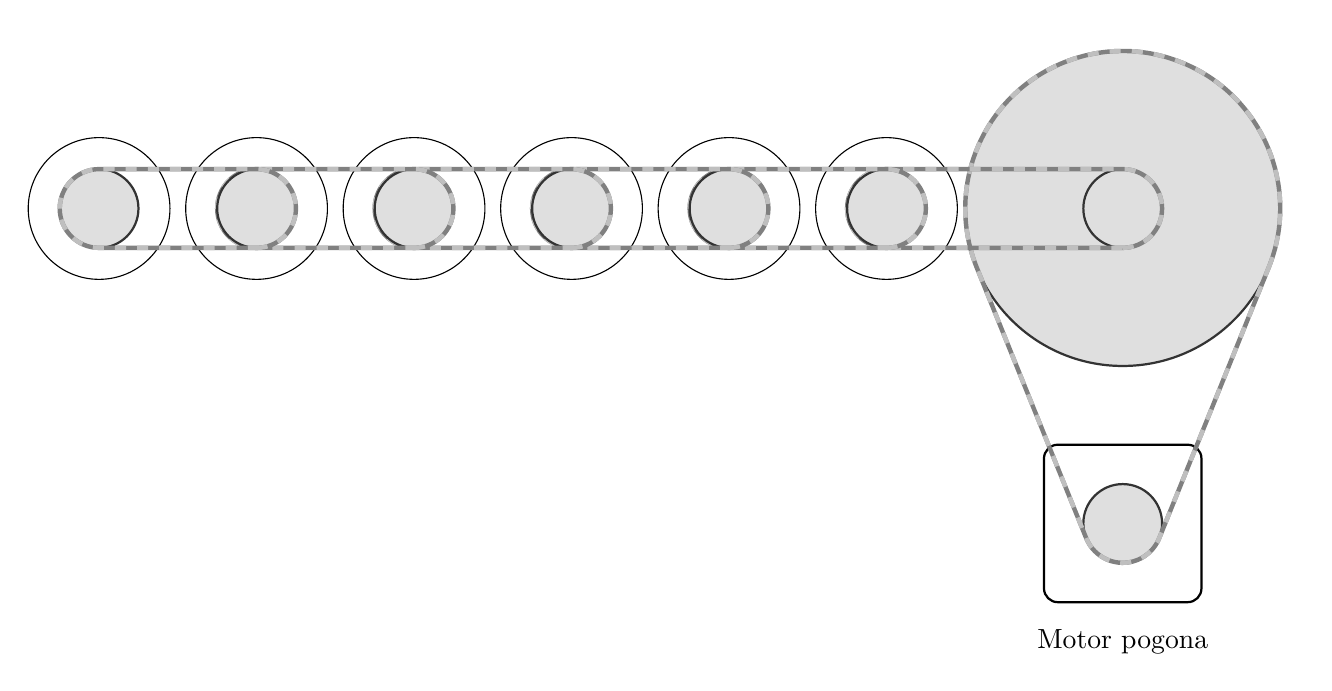
\begin{tikzpicture}[]
		\draw [ thick, rounded corners=5pt]  (5,-1) rectangle (7,-3);
		\draw[black,radius=0.9](3,2) circle; 
		\draw[black,radius=0.9](1,2) circle; 
		\draw[black,radius=0.9](-1,2) circle; 
		\draw[black,radius=0.9](-3,2) circle;
		\draw[black,radius=0.9](-5,2) circle;
		\draw[black,radius=0.9](-7,2) circle;   
		\pic {gears={size 1 at (6,-2) and size 4 at (6,2)}};
		\pic {gears={size 1 at (3,2) and size 1 at (6,2)}};
		\pic {gears={size 1 at (1,2) and size 1 at (3,2)}};
		\pic {gears={size 1 at (-1,2) and size 1 at (1,2)}};
		\pic {gears={size 1 at (-3,2) and size 1 at (-1,2)}};
		\pic {gears={size 1 at (-5,2) and size 1 at (-3,2)}};
		\pic {gears={size 1 at (-7,2) and size 1 at (-5,2)}};
		\node[] at (6,-3.5){Motor pogona};
	\end{tikzpicture}
	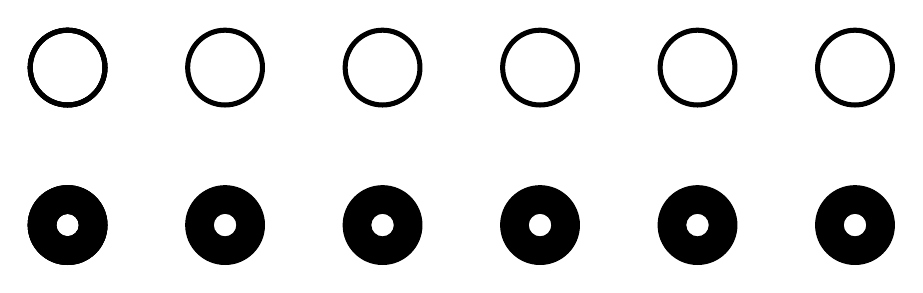
\begin{tikzpicture}[]
		\def\xPortLeft{0}
		\def\xPortRight{6}	
		\def\xKoloA{0}	
		\def\xKoloB{2}	
		\def\xKoloC{4}
		\def\xKoloD{6}
		\def\xKoloE{8}
		\def\xKoloF{10}
		\def\yKolo{1}	
		\def\yZgValj{3}
		\def\ValjInner{0.15}
		\def\ValjOuter{0.5}
				
		\def\ZgInner{0.45}	
		
		\def\xLend{2}
		\def\yTerminalBottom{1}
		\def\yLa{1.6}
		\def\yLb{0.8}
		\def\yLc{0}	
		\def\yLac{2}
		\def\yLbc{1.2}
		\def\yLcc{0.4}	
		\def\xLcrt{2.2}	
		
\draw[fill=black ,even odd rule] (\xKoloA,\yKolo) circle (\ValjOuter cm) (\xKoloA,\yKolo) circle (\ValjInner cm);
\draw[fill=black ,even odd rule] (\xKoloB,\yKolo) circle (\ValjOuter cm) (\xKoloB,\yKolo) circle (\ValjInner cm);
\draw[fill=black ,even odd rule] (\xKoloC,\yKolo) circle (\ValjOuter cm) (\xKoloC,\yKolo) circle (\ValjInner cm);\\
\draw[fill=black ,even odd rule] (\xKoloD,\yKolo) circle (\ValjOuter cm) (\xKoloD,\yKolo) circle (\ValjInner cm);\\
\draw[fill=black ,even odd rule] (\xKoloE,\yKolo) circle (\ValjOuter cm) (\xKoloE,\yKolo) circle (\ValjInner cm);\\
\draw[fill=black ,even odd rule] (\xKoloF,\yKolo) circle (\ValjOuter cm) (\xKoloF,\yKolo) circle (\ValjInner cm);\\
\draw[fill=black ,even odd rule] (\xKoloA,\yKolo) circle (\ValjOuter cm) (\xKoloA,\yKolo) circle (\ValjInner cm);
\draw[fill=black ,even odd rule] (\xKoloA,\yKolo) circle (\ValjOuter cm) (\xKoloA,\yKolo) circle (\ValjInner cm);

\draw[fill=black ,even odd rule] (\xKoloA,\yZgValj) circle (\ValjOuter cm) (\xKoloA,\yZgValj) circle (\ZgInner cm);
\draw[fill=black ,even odd rule] (\xKoloB,\yZgValj) circle (\ValjOuter cm) (\xKoloB,\yZgValj) circle (\ZgInner cm);
\draw[fill=black ,even odd rule] (\xKoloC,\yZgValj) circle (\ValjOuter cm) (\xKoloC,\yZgValj) circle (\ZgInner cm);\\
\draw[fill=black ,even odd rule] (\xKoloD,\yZgValj) circle (\ValjOuter cm) (\xKoloD,\yZgValj) circle (\ZgInner cm);\\
\draw[fill=black ,even odd rule] (\xKoloE,\yZgValj) circle (\ValjOuter cm) (\xKoloE,\yZgValj) circle (\ZgInner cm);\\
\draw[fill=black ,even odd rule] (\xKoloF,\yZgValj) circle (\ValjOuter cm) (\xKoloF,\yZgValj) circle (\ZgInner cm);\\
\draw[fill=black ,even odd rule] (\xKoloA,\yZgValj) circle (\ValjOuter cm) (\xKoloA,\yZgValj) circle (\ZgInner cm);
\draw[fill=black ,even odd rule] (\xKoloA,\yZgValj) circle (\ValjOuter cm) (\xKoloA,\yZgValj) circle (\ZgInner cm);

	\end{tikzpicture}

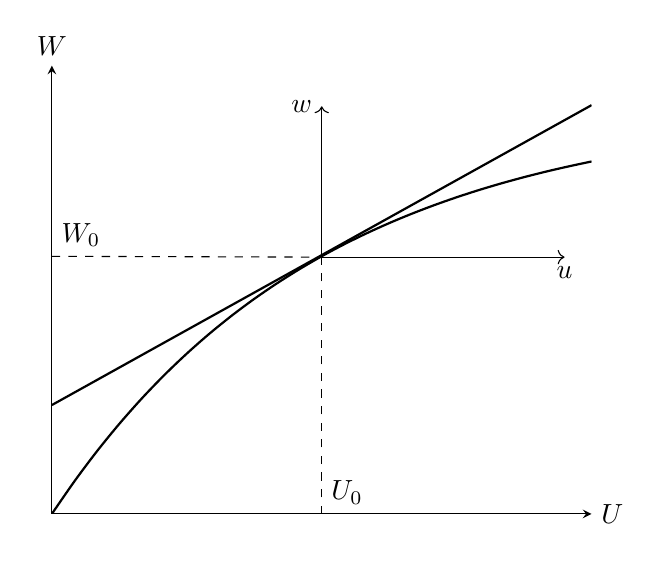
\begin{tikzpicture}
\begin{axis}[
xmin=0,
xmax=2,
ymax=1.1,
xtick = \empty,    ytick = \empty,
xlabel = {$U$},
x label style = {at={(1,0)},anchor=west},
ylabel = {$W$},
y label style = {at={(0,1)},rotate=-90,anchor=south},
axis lines=left,
%enlargelimits=1.0,
]
\addplot[color=black,smooth,thick][domain=0:2] {((x-1)*0.36787)+0.635};
\addplot[color=black,smooth,thick,-][domain=0:2] {(1-exp(-x))};
   \draw[dashed] (axis cs:0,0.632) node[above right] {$W_0$}  -- (axis cs:1,0.63);  
   \draw[dashed] (axis cs:1,0)node[above right] {$U_0$} -- (axis cs:1,0.63) ;
   \draw[->] (axis cs:1,0.63) -- (axis cs:1,1) node[left] {$w$} ;
   \draw[->] (axis cs:1,0.63)-- (axis cs:1.9,0.63) node[below] {$u$};
\end{axis}
\end{tikzpicture}

\begin{tikzpicture}
\begin{axis}[
        axis x line=middle, 
        axis y line=middle, 
xtick = \empty,    ytick = \empty,
xlabel = {$\Omega$},
ylabel = {$M,I_q$},
enlargelimits=-1.0,
]

\addplot[color=black,smooth,thick,-][domain=-0.5:3.5] {(3-x))};
\addplot[color=black,smooth,thick,-][domain=0:2] {(1)};
\filldraw[black](axis cs:3,0) circle (2pt) node[below, yshift=-0.2cm] {$\Omega_0$};
\filldraw[black](axis cs:0,3) circle (2pt) node[left, ] {$M_{zag}$};
\node[]at (axis cs:1,1.2){$I_{qn}$};
\end{axis}
\end{tikzpicture}

\begin{tikzpicture}
\begin{axis}[
xmin=0,
xmax=360,
ymax=1.1,
xtick = \empty,    ytick = \empty,
xlabel = {$U$},
x label style = {at={(1,0)},anchor=west},
ylabel = {$W$},
y label style = {at={(0,1)},rotate=-90,anchor=south},
axis lines=left,
%enlargelimits=1.0,
]
%\addplot[color=black,smooth,thick][domain=0:2] {((x-1)*0.36787)+0.635};
\addplot[color=black,smooth,thick,-][domain=10:170] {(1/sin(x)};
\draw[dashed] (axis cs:0,0.632) node[above right] {$W_0$}  -- (axis cs:1,0.63);  
\draw[dashed] (axis cs:1,0)node[above right] {$U_0$} -- (axis cs:1,0.63) ;
\draw[->] (axis cs:1,0.63) -- (axis cs:1,1) node[left] {$w$} ;
\draw[->] (axis cs:1,0.63)-- (axis cs:1.9,0.63) node[below] {$u$};
\end{axis}
\end{tikzpicture}

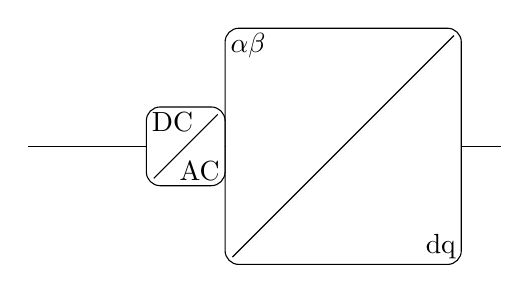
\begin{tikzpicture}[auto, node distance=2cm,>=latex']
\node[draw,convert={DC}{AC}] (a) at (0,2) {};
\node[draw,convert={ $\large\alpha\beta$}{dq}, , minimum size = 3cm] (b) at (2,2) {};
\draw (-2,2) -- (a) -- (b) -- (4,2);



\end{tikzpicture}







	

\end{document}